\documentclass[12pt,a4paper]{article}
\usepackage[brazilian]{babel}
\usepackage[utf8]{inputenc}
\usepackage{amsmath,amssymb,amsthm}
\usepackage{geometry}
\usepackage{enumitem}
\usepackage{hyperref}
\usepackage{xcolor}
\usepackage{graphicx}
\usepackage{fancyhdr}
\usepackage{tcolorbox}
\usepackage{totpages}
\usepackage{titlesec}
\usepackage{etoolbox}
\usepackage{multicol}
\usepackage{multicol}
\setlength{\columnseprule}{0.4pt} % Espessura da linha divisória
\renewcommand{\columnseprulecolor}{\color{borderlight}} % Cor da linha (opcional)

\geometry{top=3.5cm, bottom=2.5cm, left=2.0cm, right=2.0cm, headheight=2.6cm}

\definecolor{primary}{RGB}{10, 45, 90}
\definecolor{secondary}{RGB}{25, 110, 180}
\definecolor{bglight}{RGB}{245, 247, 250}
\definecolor{borderlight}{RGB}{210, 220, 230}
\definecolor{correctgreen}{RGB}{40, 140, 60}

\tcbuselibrary{skins, breakable}

\newtcolorbox{boxfixacao}[1]{
  enhanced,
  colback=bglight,
  colframe=primary,
  arc=3pt,
  boxrule=1pt,
  title={#1},
  fonttitle=\sffamily\bfseries\color{white},
  coltitle=white,
  colbacktitle=primary,
  breakable
}

\newcounter{numquestao}
\setcounter{numquestao}{0}

\newenvironment{questao}[2][]{%
  \refstepcounter{numquestao}%
  \vspace{0.3cm}%
  \begin{tcolorbox}[
    enhanced,
    colback=white,
    colframe=secondary,
    arc=2pt,
    boxrule=0.8pt,
    leftrule=4pt,
    title={\textbf{Questão \thenumquestao} \ifstrempty{#2}{}{--- #2} \hfill \small\textnormal{#1}},
    fonttitle=\sffamily\bfseries\color{white},
    coltitle=white,
    colbacktitle=secondary,
    breakable
  ]%
}{%
  \end{tcolorbox}%
}

\newenvironment{gabarito}{%
  \vspace{0.1cm}%
  \begin{tcolorbox}[
    enhanced,
    colback=bglight,
    colframe=correctgreen,
    arc=2pt,
    boxrule=0.6pt,
    title={\small\sffamily\bfseries Resolução / Gabarito},
    fonttitle=\sffamily\color{white},
    colbacktitle=correctgreen,
    breakable
  ]%
  \small
}{%
  \end{tcolorbox}%
}

\newcommand{\espacoresposta}[1]{%
  \vspace{#1}%
}

\pagestyle{fancy}
\fancyhf{}

\fancyhead[L]{%
  \small\sffamily
  \textbf{IFPE -- Campus Caruaru}
}
\fancyhead[R]{%
  \small\sffamily
  \textbf{Instituto Federal de Pernambuco -- Campus Caruaru} \\
  \textcolor{secondary}{Disciplina:} Cálculo 1 \\
  \textcolor{secondary}{Prof.:} Cleibson José da Silva
}

\fancyfoot[L]{\small\sffamily\color{gray}Lista 1 -- Exercícios de Limite}
\fancyfoot[R]{\small\sffamily\color{gray}Página \thepage\ de \ref{TotPages}}

\renewcommand{\headrulewidth}{0.8pt}
\renewcommand{\headrule}{{\color{primary}\hrule width\headwidth height \headrulewidth}}
\renewcommand{\footrulewidth}{0.4pt}

\hypersetup{
    colorlinks=true,
    linkcolor=secondary,
    urlcolor=secondary,
    citecolor=primary
}

\begin{document}

\begin{center}
  {\LARGE\bfseries\color{primary} Lista 1: Exercícios de Limite} \\[0.1cm]
  {\small\sffamily\color{gray} Exercícios de Fixação e Problemas de Limite}
\end{center}

\vspace{0.2cm}

As questões a seguir foram retiradas do livro \textit{Curso de Cálculo de Uma Variável}, Cap.1, Marco Cabral, UFRJ, 2022.

\vspace{0.3cm}

\begin{multicols*}{2}

\subsection*{Fixação}

  \begin{description}[font=\bfseries, leftmargin=0pt]
    \item[Fix 1.1:] Considere o gráfico de $y=f(x)$ esboçado abaixo. Determine os limites abaixo. Caso algum não exista, determine os limites laterais.
    
    \begin{center}
      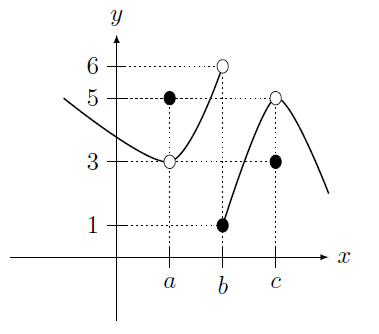
\includegraphics[width=\linewidth]{Imagens/fig1_1.png}
    \end{center}

    \begin{enumerate}[label=(\alph*)]
      \item $\displaystyle\lim_{x\to a} f(x)$
      \item $\displaystyle\lim_{x\to b} f(x)$
      \item $\displaystyle\lim_{x\to c} f(x)$
    \end{enumerate}

    \item[Fix 1.2:] Determine se é Verdadeiro ou Falso. Se for falso dê um contraexemplo ou corrija. Se for verdadeiro justifique.
        
    \begin{enumerate}[label=(\alph*)]
      \item $\{x \in \mathbb{R} \mid |x-3| \le 2\} = [1,5]$.
      \item $\{x \in \mathbb{R} \mid |x+2| < 1\} = (1,3)$.
      \item $\sqrt{x^2} = x$ para todo $x \in \mathbb{R}$.
      \item Se $g(x) = \begin{cases} 4, & x \ne 2; \\ \pi, & x = 2 \end{cases}$, então $\displaystyle\lim_{x\to 2} g(x) = g(2) = \pi$.
      \item Se $\displaystyle\lim_{x\to c} (f(x)+g(x))$ existe, então existe $\displaystyle\lim_{x\to c} f(x)$.
    \end{enumerate}

    \item[Fix 1.3:] Determine se é Verdadeiro ou Falso. Se for falso dê um contraexemplo ou corrija. Se for verdadeiro justifique.
    \begin{enumerate}[label=(\alph*)]
      \item Se $\displaystyle\lim_{x\to 3^+} f(x) = 5$, então $\displaystyle\lim_{x\to 3} f(x) = 5$.
      \item Se $\displaystyle\lim_{x\to 2} f(x) = 4$, então $\displaystyle\lim_{x\to 2^-} f(x) = -4$.
      \item Se $\displaystyle\lim_{x\to 2} f(x) = 4$, então $f(2) = 4$.
      \item Existe uma função $f$ tal que $\displaystyle\lim_{x\to 3^+} f(x) \ne \lim_{x\to 3^-} f(x) = \lim_{x\to 3} f(x)$.
      \item O gráfico de uma função pode cruzar sua assíntota horizontal.
    \end{enumerate}

    \item[Fix 1.4:] Considere a função $f(x)$ dada por 
    \[
    f(x) = \begin{cases} 5, & x \le 1 \\ 7, & 1 < x \le 2 \\ 9, & x > 2 \end{cases}
    \]
    Determine $\displaystyle\lim_{x\to k} f(x)$ ou, caso não exista, os limites laterais para:
    \begin{enumerate}[label=(\alph*), itemsep=0pt]
      \item $k=1$;
      \item $k=0.9999$;
      \item $k=1.0001$;
      \item $k=2$;
      \item $k=1.9999$;
      \item $k=2.0001$.
    \end{enumerate}

    \item[Fix 1.5:] Aplique a definição do módulo para esboçar o gráfico de:
    \begin{enumerate}[label=(\alph*)]
      \item $f(x) = \frac{\cos x}{|\cos(x)|}$
      \item $f(x) = \sqrt{|x|}$
    \end{enumerate}
  \end{description}

\subsection*{Problemas}

\begin{description}[font=\bfseries, leftmargin=0pt]
  \item[Prob 1.20:] Esboce o gráfico das seguintes funções:
  \begin{enumerate}[label=(\alph*)]
    \item $f(x) = \begin{cases} -\sqrt{9-x^2}, & |x| \le 3 \\ |x|-3, & |x| > 3 \end{cases}$
    \item $f(x) = \begin{cases} \sqrt{x-1}, & x \ge 1 \\ \log(x)+1, & x < 1 \end{cases}$
  \end{enumerate}

  \item[Prob 1.21:] Considere a função $I_{\mathbb{Z}}$ (chamada de função característica ou indicadora do conjunto $\mathbb{Z}$) definida por:
  \[
  I_{\mathbb{Z}}(x) = \begin{cases} 0, & x \notin \mathbb{Z} \\ 1, & x \in \mathbb{Z} \end{cases}
  \]
  Esboce o gráfico e determine (se existir):
  \begin{enumerate}[label=(\alph*)]
    \item $\displaystyle\lim_{x\to 3/4} I_{\mathbb{Z}}(x)$
    \item $\displaystyle\lim_{x\to -3} I_{\mathbb{Z}}(x)$
    \item $\displaystyle\lim_{x\to \infty} I_{\mathbb{Z}}(x)$
  \end{enumerate}

  \item[Prob 1.22:] Calcule os limites abaixo (quando eles existirem) justificando seus passos (sem utilizar a regra de L'Hospital). Limites com raízes:
  \begin{enumerate}[label=(\alph*)]
    \item $\displaystyle\lim_{h\to 0} \frac{\sqrt{1+h} - \sqrt{1-h}}{h}$
    \item $\displaystyle\lim_{x\to 4} \frac{|x|-4}{\sqrt{x}-2}$
    \item $\displaystyle\lim_{h\to -1} \frac{\sqrt{h^2+3}-2}{h+1}$
  \end{enumerate}

  \item[Prob 1.23:] Determine os limites e, caso não exista, os limites laterais (caso existam):
  \begin{enumerate}[label=(\alph*)]
    \item $\displaystyle\lim_{x\to -3} \sin\left(\frac{7}{x+3}\right)$
    \item $\displaystyle\lim_{x\to 2} \log|x-2|$
    \item $\displaystyle\lim_{x\to 2} \frac{|x-2|(x+1)}{x-2}$
    \item $\displaystyle\lim_{x\to -5} \frac{x+3}{x+5}$
    \item $\displaystyle\lim_{x\to 2} \frac{|x-2|}{x^2-5x+6}$
  \end{enumerate}

  \item[Prob 1.24:] Calcule os limites abaixo (quando eles existirem) justificando seus passos (sem utilizar a regra de L'Hospital):
  \begin{enumerate}[label=(\alph*)]
    \item $\displaystyle\lim_{x\to -1} \frac{x^3+1}{x+1}$
    \item $\displaystyle\lim_{x\to 2^-} \frac{x}{x^2-4}$
    \item $\displaystyle\lim_{x\to -2} \frac{x+2}{|x|-2}$
    \item $\displaystyle\lim_{x\to 1} \frac{x^4-2x^3-x+2}{x^3+2x^2-x-2}$
    \item $\displaystyle\lim_{a\to 2} \frac{(a-2)(a^2-4)}{a^3-5a^2+8a-4}$
    \item $\displaystyle\lim_{x\to 0} \left(\frac{1}{x} - \frac{1}{x^2}\right)$
    \item $\displaystyle\lim_{x\to 2} \frac{x^2-3x+2}{x^2-3x+5}$
    \item $\displaystyle\lim_{x\to 1^+} \frac{x+3}{1-x}$
    \item $\displaystyle\lim_{x\to 1} \frac{x+1-\frac{2}{x}}{x-1}$
    \item $\displaystyle\lim_{x\to -1} \frac{x^2+2x+1}{x+1}$
  \end{enumerate}
\end{description}

\end{multicols*}

\end{document}